\chapter{Discussion}\label{ch:discussion}

In our results presented in chapter \ref{ch:results} we see that our model can localise and detect anomalies. However, our models do not perform like those from \cite{pirnay_inpainting_2021} and some images have particularly low scores. This chapter reflects on those results. We also discuss some of the choices made for the experimental setup introduced in chapter \ref{ch:experimental-setup}.

\iffalse
\begin{itemize}
    \item Speed of linear model
    \item Dataset masks influencing results
    \item Equation 7?
    \item Augmentations
\end{itemize}
\fi

\section{Training data}

\subsection{Ground truth masks}

In section \ref{sec:experimental-setup:data} we introduced the MVTec AD dataset for usage in our experiment.

\begin{figure}[ht!]
\centering
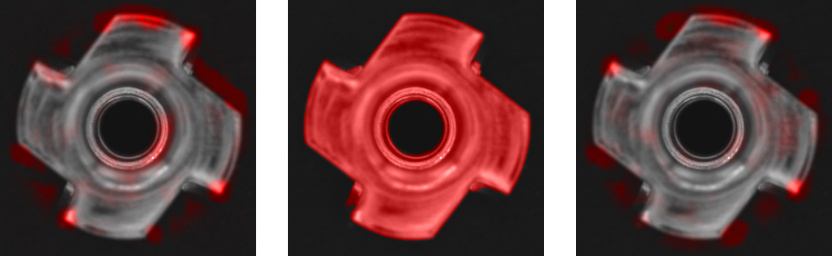
\includegraphics[width=\textwidth]{imgs/samples/metal-nut_flip_anomap.jpg}
\caption{Example of an anomalous 'flipped' image from the metal nut category comparing MSA, the dataset mask and MLSA}
\label{fig:discussion:metal-nut-anomap}
\end{figure}

In figure \ref{fig:discussion:metal-nut-anomap} we see an example of the mask compared to the parts of the images indicated as anomalous by our models. Since our models create an anomaly map that is focused on comparing the original anomalous image with a reconstruction we can only mark parts of the image that are different. The centre of these images is not different when compared to non-anomalous images. This means that our models are unable to mark the complete image as the anomaly. This could explain why the segmentation is relatively low, since the anomaly map is compared to the ground truth that does mark the complete image.

In the case of the transistor category we see a similar result. However, since the category contains multiple situations (rotations, completely missing transistors, non-centred transistors) the effect is less noticeable in the results. In figure \ref{fig:discussion:transistor-anomap} we can see that the anomaly map only matches the parts that are not present in both the original image and the reconstruction, similar to the anomaly map of the metal nut category.

\begin{figure}[ht!]
\centering
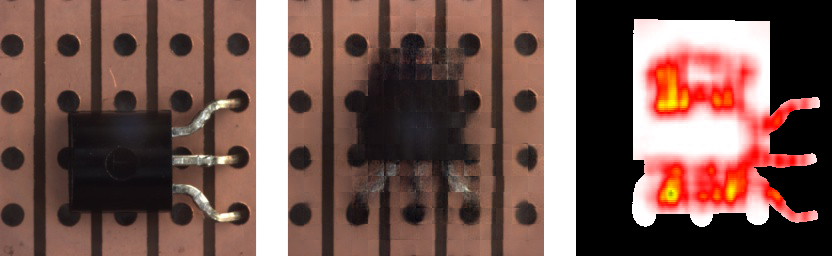
\includegraphics[width=\textwidth]{imgs/samples/transistor_misplaced_anomap.jpg}
\caption{Example of an anomalous 'misplaced' image from the transistor category showing the original image, a reconstruction and the anomaly map on top of on the ground truth mask}
\label{fig:discussion:transistor-anomap}
\end{figure}

With this knowledge we would argue that our models would never be able to reach perfect segmentation and these categories should thus be considered as hard cases. The segmentation of these anomalies would require knowledge about the object in the image.

\subsection{Data augmentations}

In \cite{pirnay_inpainting_2021} the authors mentioned using random rotation and flipping to augment the dataset during training. We have tried to implement both random rotations, vertical and horizontal flipping for our models. However, this would severely impact the results of the models, in most cases blocking them from learning to reconstruct any image. Based on the results from Pirnay et al. we think that the right augmentations could improve training the model. This would require tuning these parameters to find the correct degree of rotations.

\section{Anomaly map}

The evaluation of our models uses the anomaly map introduced in section \ref{subsec:experimental-setup:anomaly-map}. Examples of the results produced by equation \ref{eq:experimental-setup:anomap} have been shown already in figures \ref{fig:results:leather-anomap}, \ref{fig:results:grid-anomap}, \ref{fig:discussion:metal-nut-anomap} and \ref{fig:discussion:metal-nut-anomap}.

We have seen that some results only show very small parts of our images as anomaly. Since we use equation \ref{eq:experimental-setup:anomap} to remove the average reconstruction error we might be losing information. Therefore we compare our anomaly map directly to the MSGMS-map (equation \ref{eq:experimental-setup:diff}) in figures \ref{fig:discussion:bottle-msgms}, \ref{fig:discussion:metal-nut-msgms} and \ref{fig:discussion:carpet-msgms}.

These images show us that the anomaly map differs from the MSGMS-map. However, the difference is not the same for all the image categories. In the case of the bottle category the anomaly map is missing information. For the carpet category both the MSGMS-map and the anomaly map are similar. Lastly the metal nut shows us a MSGMS-map that is the complete image.

\begin{figure}[ht!]
\centering
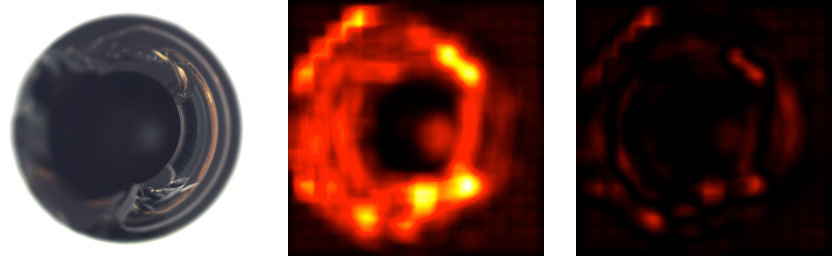
\includegraphics[width=\textwidth]{imgs/samples/bottle-ano-msgms.jpg}
\caption{Example of an anomalous image from the bottle category showing the original image, the MSGMS-map and the anomaly map}
\label{fig:discussion:bottle-msgms}
\end{figure}

\begin{figure}[ht!]
\centering
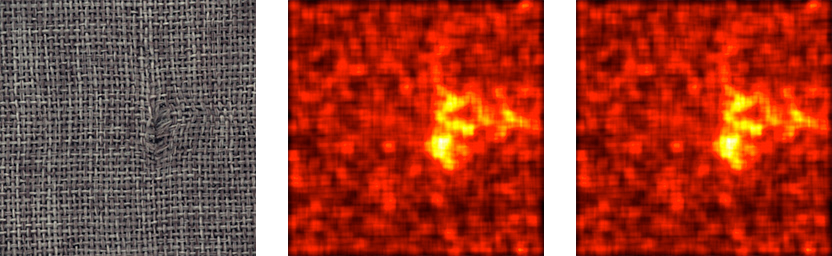
\includegraphics[width=\textwidth]{imgs/samples/carpet-ano-msgms.jpg}
\caption{Example of an anomalous image from the carpet category showing the original image, the MSGMS-map and the anomaly map}
\label{fig:discussion:carpet-msgms}
\end{figure}

\begin{figure}[ht!]
\centering
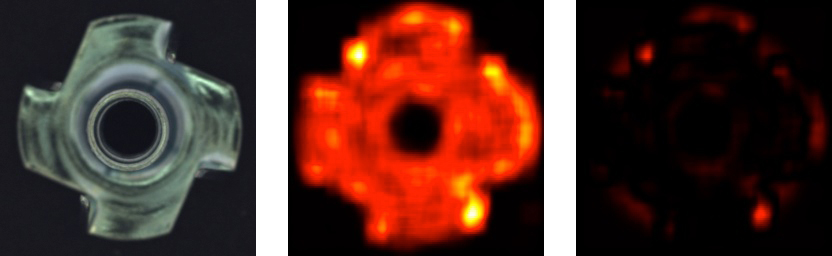
\includegraphics[width=\textwidth]{imgs/samples/metal-nut-ano-msgms.jpg}
\caption{Example of an anomalous image from the metal nut category showing the original image, the MSGMS-map and the anomaly map}
\label{fig:discussion:metal-nut-msgms}
\end{figure}

The anomaly map is created by using the average MSGMS-map over the training data. The difference we see could be the result of a high error rate over the good images. Therefore we look at some images in the test data that have no anomalies.

\begin{figure}[ht!]
\centering
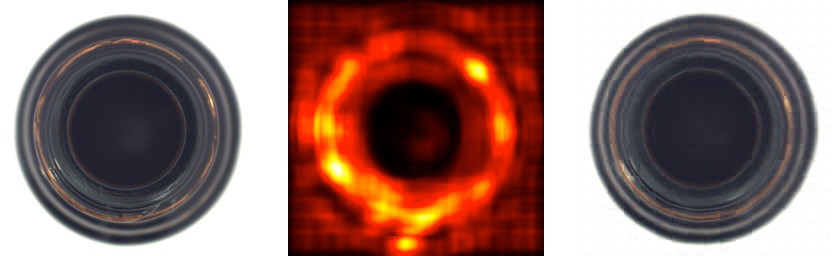
\includegraphics[width=\textwidth]{imgs/samples/bottle-good.jpg}
\caption{Comparison of a good image from the bottle category with the reconstruction and the MSGMS-map}
\label{fig:discussion:bottle-good}
\end{figure}

\begin{figure}[ht!]
\centering
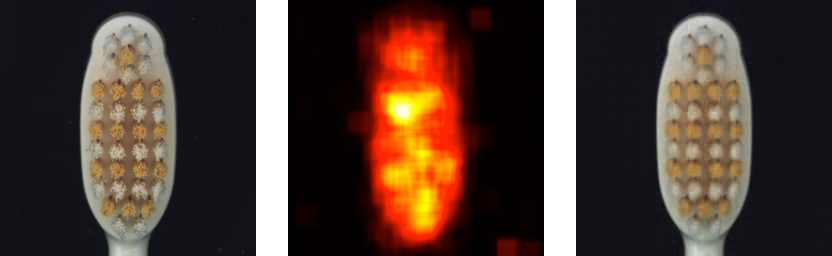
\includegraphics[width=\textwidth]{imgs/samples/toothbrush-good.jpg}
\caption{Comparison of a good image from the toothbrush category with the reconstruction and the MSGMS-map}
\label{fig:discussion:toothbrush-good}
\end{figure}

In figure \ref{fig:discussion:bottle-good} and \ref{fig:discussion:toothbrush-good} we see that for the good images we also have version of a MSGMS-map that could indicate an anomaly that is not present. This means that directly using the MSGMS-map could improve the scores for segmentation. However, since we are using the max pixel value for the detection of anomalies in images this would mean that all images would contain an anomaly. That would severely hurt the performance.

We thus need to use the average error during training to post-process our MSGMS-map that is created by comparing the original images to the reconstructions. The reconstructions that our models make are not sufficiently detailed enough for our MSGMS-map to not spot any differences.

An alternative to using the average training error would be to determine a threshold. This would allow us to remove values below the threshold. This does require that extra step and would require a different value for each image. In contrast, the current solution can be a compromise for the large range of image types in the dataset.

\section{Model efficiency}

In section \ref{sec:results:efficiency} we answered our research questions regarding the efficiency of the MSA and MLSA models. We saw that the time taken per epoch is lower for MSA when compared to MLSA. However, the paper by Katharopoulos et al. \cite{katharopoulos_transformers_2020} that introduced MLSA reports a significant difference in the time taken for each epoch in favour of MLSA.

Even though the MLSA models require less epochs for training on average, we would still expect the MLSA based models to take less time for each epoch.

The first reason for this difference could be an implementation error of the linear attention function. Our transformers are based on a library\footnote{https://github.com/idiap/fast-transformers} by Katharopoulos et al. that contains multiple attention implementations. It allows the user to select a type of transformer, or a part of the transformer structure, and build a model around it. Since we use this library we think it is unlikely that the implementation of the attention function causes the time difference of our model. Moreover, the time difference between running the two attention types is verifiable by running the basic example from the repository. We have done this on the cluster machines, giving us 87.59ms versus 54.43ms for the normal and linear attention functions respectively.

A second cause for the differences could be the code surrounding the attention function. Primarily loading the images from disk and splitting them into patches can be resource intensive. Similarly the loss function can take a longer time to calculate. To be able to figure out the resource usage of each part in our model we would need to run our models with a profiler. This is something that could be a good starting point for future work since a job with a profiler uses a lot more resources, based on the (failed) test runs that we have done.

To make sure that the difference in time per epoch is not something that we only observe for long jobs we have executed a training run with one epoch for the carpet image. This gave us a training time of 1:36:41 for MSA and 1:54:22 for MLSA. Which is a higher difference than the one we see in table \ref{table:results:times}, but still favours MSA as well.